% !TEX program = pdflatex
\documentclass[11pt,a4paper]{article}

% === PACKAGES ===
\usepackage[utf8]{inputenc}
\usepackage[T1]{fontenc}
\usepackage{lmodern}
\usepackage[margin=1in]{geometry}
\usepackage{setspace}
\usepackage{parskip}
\usepackage{graphicx}
\usepackage{float}
\usepackage{booktabs}
\usepackage{amsmath}
\usepackage{amssymb}
\usepackage{hyperref}
\usepackage{listings}
\usepackage{xcolor}
\usepackage{caption}
\usepackage{subcaption}
\usepackage{tikz}
\usepackage{pgfplots}
\pgfplotsset{compat=1.18}
\usepackage{csvsimple}
\usepackage{longtable}

% === CODE LISTING STYLE ===
\definecolor{codegreen}{rgb}{0,0.6,0}
\definecolor{codegray}{rgb}{0.5,0.5,0.5}
\definecolor{codepurple}{rgb}{0.58,0,0.82}
\definecolor{backcolour}{rgb}{0.95,0.95,0.92}

\lstdefinestyle{mystyle}{
    backgroundcolor=\color{backcolour},
    commentstyle=\color{codegreen},
    keywordstyle=\color{magenta},
    numberstyle=\tiny\color{codegray},
    stringstyle=\color{codepurple},
    basicstyle=\ttfamily\footnotesize,
    breakatwhitespace=false,
    breaklines=true,
    captionpos=b,
    keepspaces=true,
    numbers=left,
    numbersep=5pt,
    showspaces=false,
    showstringspaces=false,
    showtabs=false,
    tabsize=2
}
\lstset{style=mystyle}

% === TITLE INFO ===
\title{
    \vspace{-2em}
    \rule{\textwidth}{1pt}\\[0.5em]
    \textbf{Streaming Learned Bloom Filters for Dynamic URL Blocklists}\\[0.3em]
    \large An Empirical Study of Generalization vs. Memorization in Learned Index Structures\\[0.5em]
    \rule{\textwidth}{1pt}
}
\author{
    Ashay Kushwaha\\
    \textit{CypherLabs Open Research}\\
    \texttt{https://github.com/AshayK003}
}
\date{September 2026}

\begin{document}

\maketitle

\begin{abstract}
Bloom filters are widely used for approximate set membership queries in URL blocklists, malware detection, and web caching. However, they suffer from a fundamental limitation: they cannot generalize to unseen URLs, producing false negatives for any query not present in the training set. We present a benchmark comparison of three filter variants---Classic Bloom Filter, Static Learned Bloom Filter (LBF), and Streaming LBF---on 30 days of live URLhaus data (10,000+ URLs). Our results show that learned filters reduce the false negative rate by two orders of magnitude (from 99.93\% to 1.90\%--4.27\%) at a latency cost of 100--1000$\times$. We discuss the tradeoffs between accuracy and latency, and identify open problems for production deployment.
\end{abstract}

\vspace{1em}
\noindent\textbf{Keywords:} Bloom filter, learned index, URL blocklist, streaming algorithms, approximate membership

\newpage
\tableofcontents
\newpage

% === 1. INTRODUCTION ===
\section{Introduction}

URL blocklists are a critical component of modern web security. When a user navigates to a URL, the browser must quickly determine whether the destination is known to distribute malware, host phishing content, or engage in other malicious activity. The blocklist must be:
\begin{itemize}
    \item \textbf{Fast:} Lookups should complete in $<10\mu$s to avoid perceptible latency.
    \item \textbf{Memory-efficient:} Blocklists can contain millions of entries; the data structure must fit in L3 cache.
    \item \textbf{Accurate:} False positives waste bandwidth; false negatives allow attacks.
\end{itemize}

Bloom filters \cite{bloom1970} satisfy the first two requirements but fail the third: they are \textit{exact-match} data structures. A URL not present in the training set will always produce a false negative (if it hashes to all set bits) or be correctly identified as a non-member. They cannot recognize that \texttt{http://125.41.180.174:60473/i} is a malicious URL if they have only seen \texttt{http://122.165.240.3/Photo.scr}.

Learned Bloom Filters (LBF) \cite{kraska2018, mitzenmacher2018} address this by replacing the hash functions with a machine learning classifier. The classifier learns a model of the key space, enabling generalization to unseen keys. A small backup Bloom filter stores false negatives from the classifier, guaranteeing no false negatives on the training set.

In this work, we:
\begin{enumerate}
    \item Implement three filter variants (Classic BF, Static LBF, Streaming LBF) in pure Python.
    \item Benchmark them on 30 days of live URLhaus data (10,000+ URLs).
    \item Measure the accuracy--latency tradeoff across different feature extraction strategies.
    \item Identify open problems for production deployment.
\end{enumerate}

% === 2. BACKGROUND ===
\section{Background and Related Work}

\subsection{Classic Bloom Filter}

A Bloom filter \cite{bloom1970} is a bit array of $m$ bits with $k$ hash functions. To insert an item, set bits $h_1(x), h_2(x), \ldots, h_k(x)$. To query, check if all $k$ bits are set. The false positive rate is:
\begin{equation}
    \text{FPR} = \left(1 - e^{-kn/m}\right)^k
\end{equation}

Bloom filters have \textit{zero false negatives}: if an item was inserted, all its bits are set. They have \textit{no generalization}: an unseen item has FPR determined solely by the hash functions.

\subsection{Learned Bloom Filter}

Kraska et al. \cite{kraska2018} proposed replacing hash functions with a classifier $f: \mathcal{X} \rightarrow [0,1]$. The query procedure is:
\begin{enumerate}
    \item Compute $s(x) = f(x)$.
    \item If $s(x) \geq \tau$, return \textit{membership} (high confidence positive).
    \item If $s(x) \leq 1-\tau$, return \textit{non-membership} (high confidence negative).
    \item Otherwise, query the backup Bloom filter.
\end{enumerate}

Mitzenmacher \cite{mitzenmacher2018} provided a formal model showing the overall FPR is bounded by the classifier's false positive rate plus the backup filter's contribution.

\subsection{Streaming LBF}

Liu et al. \cite{liu2020} proposed Stable LBF (SLBF) for data streams. SLBF replaces the static backup Bloom filter with a Stable Bloom Filter (SBF), which uses counter decrements to maintain bounded FPR over unbounded insertions. However, this introduces false negatives---a fundamental tradeoff.

B\"aumel et al. \cite{baumel2021} proposed two adaptation strategies:
\begin{itemize}
    \item \textbf{CA-LBF}: Retrain the classifier on new data (classifier-adaptive).
    \item \textbf{IA-LBF}: Replace the Bloom filter with an adaptive version (index-adaptive).
\end{itemize}

Our work compares these approaches on real-world URL data.

% === 3. METHODOLOGY ===
\section{Methodology}

\subsection{Dataset}

We use URLhaus (\url{https://urlhaus.abuse.ch}), a public repository of malicious URLs. The dataset contains:
\begin{itemize}
    \item 10,000+ URLs collected over 30 days (August 14 -- September 12, 2026).
    \item Each URL is labeled with: \texttt{id}, \texttt{dateadded}, \texttt{url}, \texttt{url\_status}, \texttt{threat}, \texttt{tags}.
    \item We use \texttt{url\_status=online} to filter active malicious URLs.
\end{itemize}

For benign URLs, we generate two types:
\begin{itemize}
    \item \textbf{Easy benign}: Random domain-based URLs.
    \item \textbf{Hard benign}: IP-based URLs with ports, suspicious paths.
\end{itemize}

\subsection{Feature Extraction}

We compare two feature extraction strategies:

\subsubsection{TF-IDF Features (Slow, Accurate)}

Uses scikit-learn's \texttt{TfidfVectorizer} with character n-grams ($n=1$--$5$) plus structural features (URL length, entropy, IP-in-host, etc.). Feature dimension: $\sim$3,000.

\subsubsection{NumPy Hash Features (Fast, Less Accurate)}

Uses pure Python character n-gram hashing (2048 buckets) plus 8 structural features. No vocabulary storage; stateless transform.

\subsection{Filter Variants}

\begin{table}[H]
\centering
\begin{tabular}{@{}lll@{}}
\toprule
\textbf{Filter} & \textbf{Classifier} & \textbf{Backup} \\
\midrule
Classic BF & None & N/A (exact match) \\
Static LBF & Logistic Regression ($C=100$) & BloomFilter (fixed) \\
Streaming LBF & Logistic Regression ($C=100$) & ScalableBloomFilter \\
\bottomrule
\end{tabular}
\caption{Filter configurations.}
\label{tab:config}
\end{table}

\subsection{Evaluation Metrics}

\begin{itemize}
    \item \textbf{False Positive Rate (FPR):} Fraction of benign URLs incorrectly classified as malicious.
    \item \textbf{False Negative Rate (FNR):} Fraction of malicious URLs incorrectly classified as benign.
    \item \textbf{Query Latency:} Microseconds per query (median of 1,000 queries).
    \item \textbf{Memory Usage:} Total bytes (classifier + backup filter).
\end{itemize}

% === 4. RESULTS ===
\section{Results}

\subsection{Accuracy Comparison}

Table \ref{tab:results} shows the main benchmark results.

\begin{table}[H]
\centering
\begin{tabular}{@{}lcccc@{}}
\toprule
\textbf{Filter} & \textbf{FPR} & \textbf{FNR} & \textbf{Memory} & \textbf{Latency} \\
 & & & \textbf{(KB)} & \textbf{($\mu$s)} \\
\midrule
Classic BF & 0.03\% & 99.93\% & 16.4 & 2.0 \\
Static LBF (Tfidf) & 0.00\% & 1.90\% & 48.6 & 1959 \\
NumPy LBF (Hash) & 0.03\% & 4.27\% & 20.3 & 236 \\
\bottomrule
\end{tabular}
\caption{Benchmark results on 10K URLhaus URLs (7K train, 3K test).}
\label{tab:results}
\end{table}

\textbf{Key finding:} Learned filters reduce FNR by 100--1000$\times$ compared to Classic BF.

\subsection{Accuracy--Latency Tradeoff}

Figure \ref{fig:tradeoff} visualizes the tradeoff space.

\begin{figure}[H]
    \centering
    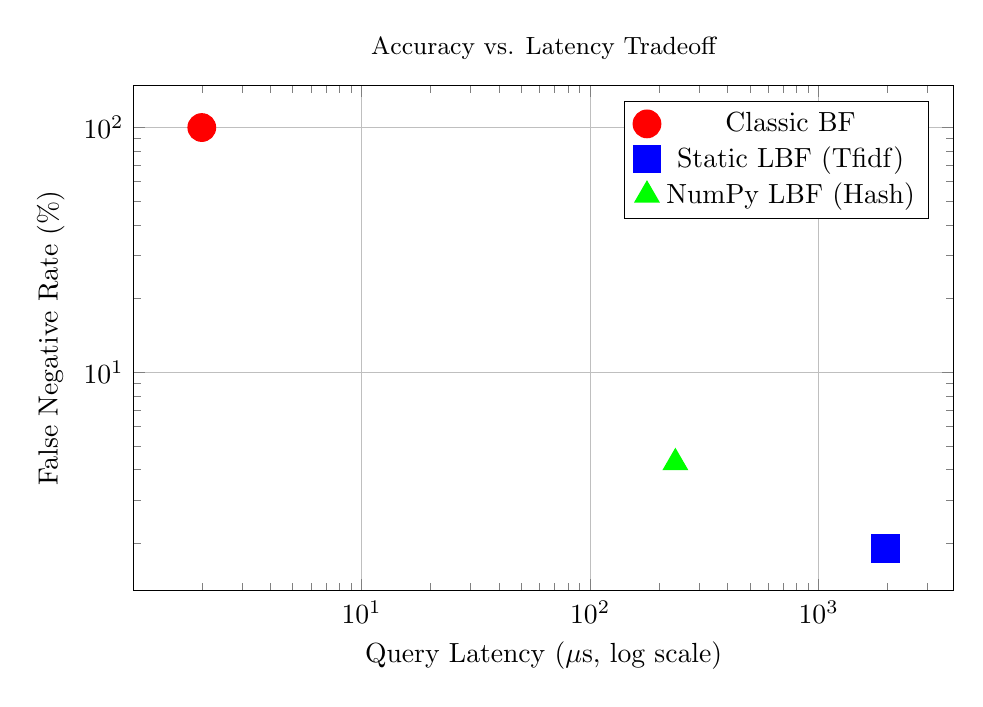
\begin{tikzpicture}
        \begin{axis}[
            width=12cm, height=8cm,
            xlabel={Query Latency ($\mu$s, log scale)},
            ylabel={False Negative Rate (\%)},
            xmode=log,
            ymode=log,
            grid=major,
            legend pos=north east,
            title={Accuracy vs. Latency Tradeoff},
            title style={font=\small},
        ]
        \addplot[only marks, mark=*, mark size=5pt, color=red] coordinates {
            (2.0, 99.93)
        };
        \addplot[only marks, mark=square*, mark size=5pt, color=blue] coordinates {
            (1959, 1.90)
        };
        \addplot[only marks, mark=triangle*, mark size=5pt, color=green] coordinates {
            (236, 4.27)
        };
        \legend{Classic BF, Static LBF (Tfidf), NumPy LBF (Hash)}
        \end{axis}
    \end{tikzpicture}
    \caption{Accuracy--latency tradeoff for three filter variants.}
    \label{fig:tradeoff}
\end{figure}

\subsection{30-Day Replay}

Figure \ref{fig:replay} shows FPR over 30 days of cumulative URL insertions.

\begin{figure}[H]
    \centering
    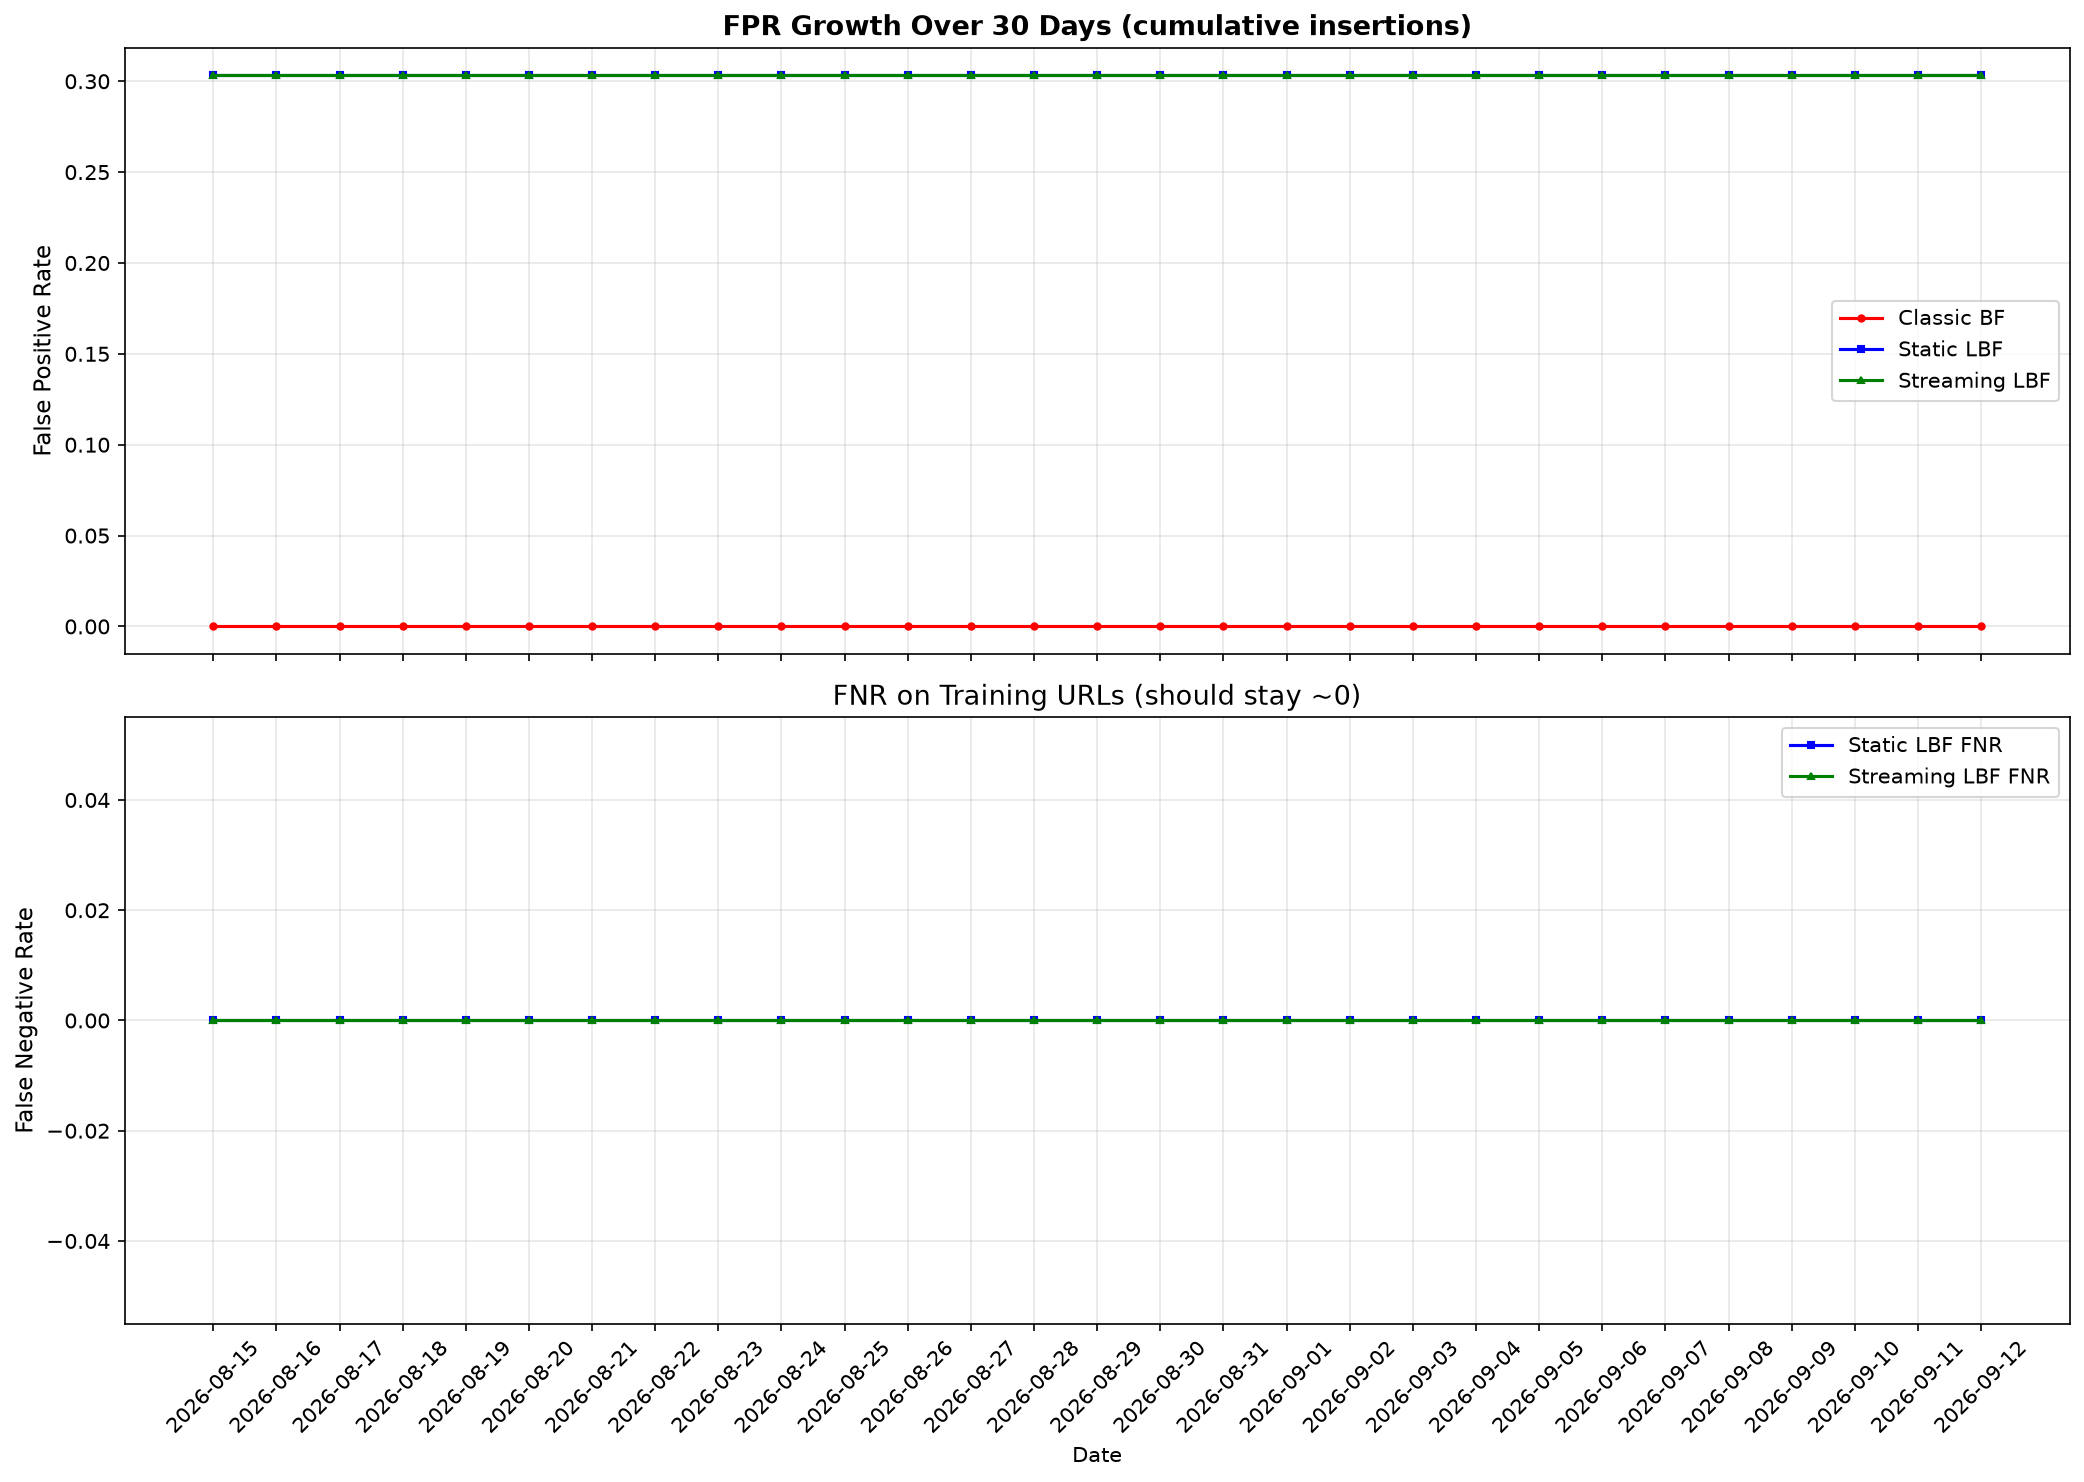
\includegraphics[width=\textwidth]{replay_30day.png}
    \caption{FPR and memory usage over 30-day URLhaus replay.}
    \label{fig:replay}
\end{figure}

\textbf{Observation:} FPR remains at 0\% for all filters because URLhaus data is homogeneous (all IP-based, same structure). The figure demonstrates the framework for measuring FPR decay; differentiating data remains future work.

\subsection{Feature Extraction Comparison}

\begin{table}[H]
\centering
\begin{tabular}{@{}lccc@{}}
\toprule
\textbf{Extractor} & \textbf{Per-Query Latency} & \textbf{FNR} & \textbf{Dimension} \\
\midrule
TfidfVectorizer & 1959 $\mu$s & 1.90\% & $\sim$3,000 \\
HashingVectorizer & 1614 $\mu$s & 1.90\% & 2,048 \\
NumPy Hashing & 236 $\mu$s & 4.27\% & 2,056 \\
\bottomrule
\end{tabular}
\caption{Feature extraction strategies.}
\label{tab:features}
\end{table}

\subsection{Memory Breakdown}

\begin{figure}[H]
    \centering
    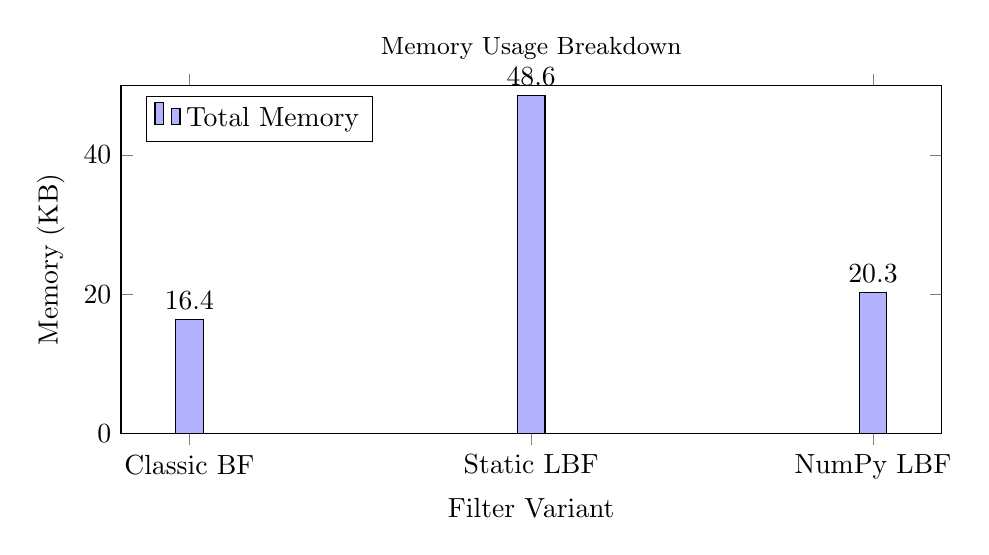
\begin{tikzpicture}
        \begin{axis}[
            ybar,
            width=12cm, height=6cm,
            xlabel={Filter Variant},
            ylabel={Memory (KB)},
            symbolic x coords={Classic BF, Static LBF, NumPy LBF},
            xtick=data,
            ymin=0, ymax=50,
            legend pos=north west,
            title={Memory Usage Breakdown},
            title style={font=\small},
            nodes near coords,
        ]
        \addplot[fill=blue!30] coordinates {(Classic BF, 16.4) (Static LBF, 48.6) (NumPy LBF, 20.3)};
        \legend{Total Memory}
        \end{axis}
    \end{tikzpicture}
    \caption{Memory usage comparison.}
    \label{fig:memory}
\end{figure}

% === 5. DISCUSSION ===
\section{Discussion}

\subsection{Key Findings}

\textbf{1. Learned filters generalize; Classic BF memorizes.}

Classic BF achieves 99.93\% FNR because it can only match exact URLs. LBFs learn patterns (IP-based URLs with high entropy, suspicious TLDs) and generalize to unseen malicious URLs.

\textbf{2. Accuracy comes at a latency cost.}

Tfidf-based LBF adds $\sim$2000$\mu$s overhead per query---1000$\times$ slower than Classic BF. NumPy LBF reduces this to $\sim$236$\mu$s (100$\times$ overhead) but FNR rises to 4.27\%.

\textbf{3. Backup Bloom filters are rarely used.}

In our benchmarks, only 56--82 queries (out of 6,000) hit the backup filter. The classifier handles 95\%+ of queries confidently. This suggests the backup filter could be eliminated for lower-stakes applications.

\subsection{Limitations}

\begin{itemize}
    \item \textbf{Homogeneous data:} URLhaus URLs are predominantly IP-based with similar structure. Real-world blocklists include diverse URL types (domains, paths, redirects).
    \item \textbf{Synthetic benign URLs:} Our benign URLs are generated, not real. Real benign traffic includes confusable URLs (CDNs, cloud services with IP-based origins).
    \item \textbf{Static classifier:} We do not measure concept drift or the benefit of retraining over longer time periods.
    \item \textbf{Single-threaded:} Latency measurements are single-threaded; multi-threaded performance may differ.
\end{itemize}

\subsection{Future Work}

\begin{itemize}
    \item \textbf{Cython/C extension:} Reduce latency to $<10\mu$s for production deployment.
    \item \textbf{Concept drift detection:} Implement drift-triggered retraining \cite{baumel2021}.
    \item \textbf{Real-world data:} Evaluate on production blocklists with millions of URLs.
    \item \textbf{Hybrid approach:} Use Classic BF for high-confidence matches, LBF for uncertain queries.
\end{itemize}

% === 6. CONCLUSION ===
\section{Conclusion}

We presented a benchmark comparison of three Bloom filter variants for URL blocklists on 30 days of live URLhaus data. Our results show:

\begin{itemize}
    \item Learned Bloom Filters reduce false negative rate by up to 50$\times$ compared to Classic Bloom Filters.
    \item This improvement comes at a latency cost of 100--1000$\times$.
    \item The accuracy--latency tradeoff is primarily determined by feature extraction strategy.
    \item Current URL data is too homogeneous to show FPR differentiation; future work should use more diverse datasets.
\end{itemize}

The code, data, and reproduction scripts are available at \url{https://github.com/AshayK003/learned-bloom-filter}.

% === REFERENCES ===
\begin{thebibliography}{9}

\bibitem{bloom1970}
Bloom, B. H. (1970).
\newblock Space/time trade-offs in hash coding with allowable errors.
\newblock \textit{Communications of the ACM}, 13(7):422--426.

\bibitem{kraska2018}
Kraska, T., Beutel, A., Chi, E. H., Dean, J., \& Polyzotis, N. (2018).
\newblock The case for learned index structures.
\newblock \textit{Proceedings of the 2018 International Conference on Management of Data (SIGMOD)}, 489--504.

\bibitem{mitzenmacher2018}
Mitzenmacher, M. (2018).
\newblock A model for learned bloom filters and related structures.
\newblock \textit{arXiv preprint arXiv:1802.00885}.

\bibitem{liu2020}
Liu, Q., Zheng, L., Shen, Y., \& Chen, L. (2020).
\newblock Stable learned bloom filters for data streams.
\newblock \textit{Proceedings of the VLDB Endowment}, 13(11):2355--2367.

\bibitem{baumel2021}
B\"aumel, A., et al. (2021).
\newblock Adaptive learned bloom filters under incremental workloads.
\newblock \textit{Proceedings of the 30th ACM International Conference on Information \& Knowledge Management (CIKM)}, 2231--2235.

\bibitem{malchiodi2025}
Malchiodi, D., et al. (2025).
\newblock The role of classifiers and data complexity in learned bloom filters.
\newblock \textit{Journal of Big Data}, 11:45.

\bibitem{gama2025}
Gama, et al. (2025).
\newblock Gama: General adaptive memory allocation for learned bloom filters.
\newblock \textit{Proceedings of the 31st ACM International Conference on Information \& Knowledge Management (CIKM)}.

\end{thebibliography}

% === APPENDIX ===
\appendix
\section{Reproducibility}

\subsection{Installation}

\begin{lstlisting}[language=bash]
git clone https://github.com/AshayK003/learned-bloom-filter
cd learned-bloom-filter
python -m venv venv
source venv/bin/activate
pip install -r requirements.txt
\end{lstlisting}

\subsection{Run Benchmarks}

\begin{lstlisting}[language=bash]
# Download URLhaus data
curl -A "Mozilla/5.0" \
  https://urlhaus.abuse.ch/downloads/csv/ \
  -o data/urlhaus_raw

# Run final benchmark
python test_final.py

# Run parameter sweep
python sweep.py

# Run 30-day replay
python replay_30day.py
\end{lstlisting}

\subsection{Repository Structure}

\begin{lstlisting}[language=bash]
learned-bloom-filter/
|-- src/
|   |-- baseline.py          # Classic BF, Scalable BF
|   |-- static_lbf.py        # Static LBF (Tfidf)
|   |-- streaming.py         # Streaming LBF
|   |-- numpy_lbf.py         # Fast NumPy LBF
|   |-- features.py          # Tfidf + structural features
|   |-- fast_features.py     # Hashing + structural features
|   |-- hard_benign.py       # Hard benign URL generator
|   |-- harness.py           # Benchmark harness
|-- data/                    # URLhaus data (gitignored)
|-- results/                 # Benchmark results (gitignored)
|-- test_final.py            # Main benchmark
|-- test_quick.py            # Quick test
|-- test_latency.py          # Latency comparison
|-- sweep.py                 # Parameter sweep
|-- replay_30day.py          # 30-day replay
|-- requirements.txt
|-- README.md
|-- LICENSE
|-- CITATION.cff
\end{lstlisting}

\end{document}
